\documentclass[sigplan,10pt]{acmart}

\usepackage[T1]{fontenc}
\usepackage[utf8]{inputenc}

\usepackage{acronym} % \ac[p], \acl[p], \acs[p], \acf[p]
\usepackage{algorithm} % \begin{algorithm} \end{algorithm}
\usepackage{algpseudocode} % \begin{algorithmic} \end{algorithmic}
\algnewcommand{\LeftComment}[1]{$\triangleright$ #1}

\usepackage[inline]{enumitem} % \begin{enumerate*} \end{enumerate*}
\usepackage{tikz} % \begin{tikzpicture} \end{tikzpicture}

\usepackage{graphicx}
\usepackage{color}
\AtBeginDocument{
\definecolor{pdfurlcolor}{rgb}{0,0,0}
\definecolor{pdfcitecolor}{rgb}{0,0,0}
\definecolor{pdflinkcolor}{rgb}{0,0,0}
\definecolor{light}{gray}{.85}
\definecolor{vlight}{gray}{.95}
\definecolor{darkgreen}{rgb}{0.0, 0.2, 0.13}
\definecolor{mydarkblue}{RGB}{116,173,209}
\definecolor{mydarkblueid}{RGB}{83,154,198}
\definecolor{mylightblue}{RGB}{171,217,233}
\definecolor{mydarkorange}{RGB}{244,109,67}
\definecolor{mylightorange}{RGB}{252,153,54}
\definecolor{mydarkred}{RGB}{215,48,39}
}


\usepackage[draft,inline,nomargin,index]{fixme}
\fxsetup{theme=colorsig,mode=multiuser,inlineface=\itshape,envface=\itshape}
\FXRegisterAuthor{go}{ago}{Gerald}
\FXRegisterAuthor{mn}{amn}{Matthieu}

\usepackage{subcaption} % subfigure

% Commands
%---------
\newcommand{\ie}{i.e. }

\newcommand{\inbb}[1]{\in \mathbb{#1}}
\newcommand{\mathlist}[2]{\set{#1_i \in #2}_{i \inbb{N}}}
\newcommand{\trm}[1]{\mathit{#1}}
\newcommand{\set}[1]{\left\{#1\right\}} % set brace notation

\newcommand{\id}[3]{$\trm{#1}^{\trm{#2}}_{\trm{#3}}$}

\newcommand{\widthletter}{7mm}
\newcommand{\widthblock}{11mm}

% Tikz styles
\tikzset{
    common/.style={anchor=west, draw, rectangle, minimum height=6mm},
    letter/.style={common, minimum width=\widthletter},
    block/.style={common, minimum width=\widthblock},
    cross/.style={
        path picture={
            \draw[mydarkred, very thick]
                (path picture bounding box.south east)--(path picture bounding box.north west)
                (path picture bounding box.south west)--(path picture bounding box.north east);
        }
    }
}

% Acronyms
% --------
\acrodef{ADT}[ADT]{Abstract Data Type}
\acrodefplural{ADT}[ADTs]{Abstract Data Types}
\acrodef{CRDT}[CRDT]{Conflict-free Replicated Data Type}
\acrodefplural{CRDT}[CRDTs]{Conflict-free Replicated Data Types}
\acrodef{JIT}[JIT]{Just-In-Time}
\acrodef{OT}[OT]{Operational Transformation}
\acrodefplural{OT}[OT]{Operational Transformations}
\acrodef{P2P}[P2P]{Peer-to-Peer}
\acrodef{SEC}[SEC]{Strong Eventual Consistency}

% Additional config
% --------
\bibliographystyle{unsrtnat}
\def\algorithmautorefname{Algorithm} % \autoref
\hyphenation{Renamable-LogootSplit}

% Pre-print settings
\settopmatter{printacmref=false}
\renewcommand\footnotetextcopyrightpermission[1]{} % removes footnote with conference information in first column
\pagestyle{plain} % removes running headers

% PaPoc'20 settings
% \copyrightyear{2020}
% \acmYear{2020}
% \setcopyright{licensedothergov}\acmConference[PaPoC '20]{7th Workshop on Principles and Practice of Consistency for Distributed Data}{April 27, 2020}{Heraklion, Greece}
% \acmBooktitle{7th Workshop on Principles and Practice of Consistency for Distributed Data (PaPoC '20), April 27, 2020, Heraklion, Greece}
% \acmPrice{15.00}
% \acmDOI{10.1145/3380787.3393682}
% \acmISBN{978-1-4503-7524-5/20/04}

\begin{document}

\title{Efficient Renaming in Sequence CRDTs}

\author{Matthieu Nicolas}
\email{matthieu.nicolas@loria.fr}
\affiliation{%
  \institution{Université de Lorraine, CNRS, Inria, LORIA, F-54500}
  \city{Nancy}
  \country{France}
}

\author{Gérald Oster}
\email{gerald.oster@loria.fr}
\affiliation{%
  \institution{Université de Lorraine, CNRS, Inria, LORIA, F-54500}
  \city{Nancy}
  \country{France}
}

\author{Olivier Perrin}
\email{olivier.perrin@loria.fr}
\affiliation{%
  \institution{Université de Lorraine, CNRS, Inria, LORIA, F-54500}
  \city{Nancy}
  \country{France}
}

\begin{abstract}
\end{abstract}

\keywords{CRDTs, real-time collaborative editing, eventual consistency, memory-wise optimisation, performance}

\maketitle

\section{Introduction}

\section{Background}

\subsection{LogootSplit}

\subsection{Limits}

\section{Overview}

\subsection{Proposed approach}

We propose a new Sequence \ac{CRDT} belonging to the variable-size identifiers approach : \emph{RenamableLogootSplit} (RLS).

This new \ac{CRDT} associates to LogootSplit a renaming mechanism.
The goal of this mechanism is to overcome LogootSplit evergrowing memory overhead.
To this end, the mechanism reassigns shorter identifiers to elements and aggregates them into fewer blocks in a fully distributed manner.

We describe the behavior of the mechanism in \autoref{sec:renamablelogootsplit}.

\subsection{System Model}

\section{RenamableLogootSplit}
\label{sec:renamablelogootsplit}

\subsection{\emph{rename} operation}

\begin{algorithm}
    \caption{Rename identifier}
    \label{alg:renameId}
    \begin{algorithmic}
    \Function{renId}{$\trm{id}, \trm{renamedIds}, \trm{nId}, \trm{nSeq}$}
        \Statex \LeftComment{$\trm{id}$ is the identifier to rename}
        \Statex \LeftComment{$\trm{renamedIds}$ is the former state shared by the \emph{rename} op}
        \Statex \LeftComment{$\trm{nId}$ is $\trm{node~id}$ of the node which issued the \emph{rename} op}
        \Statex \LeftComment{$\trm{nSeq}$ is $\trm{node~seq}$ of the node which issued the \emph{rename} op}
        \\
        \State $\trm{length} \gets \trm{renamedIds.length}$
        \State $\trm{firstId} \gets \trm{renamedIds}[0]$
        \State $\trm{lastId} \gets \trm{renamedIds}[\trm{length} - 1]$
        \State $\trm{pos} \gets \trm{getPosition}(\trm{firstId})$
        \\
        \If{$\trm{id} < \trm{firstId}$}
            \State $\trm{newFirstId} \gets \trm{new} \ \trm{Id}(\trm{pos}, \trm{nId}, \trm{nSeq}, 0)$
            \State \Return $\trm{renIdLessThanFirstId}(\trm{id}, \trm{firstId}, \trm{newFirstId})$
        \ElsIf{$\trm{id} \in \trm{renameIds}$}
            \State $\trm{index} \gets \trm{findIndex}(\trm{id}, \trm{renamedIds})$
            \State \Return $\trm{renIdFromIndex}(\trm{pos}, \trm{nId}, \trm{nSeq}, \trm{index})$
        \ElsIf{$\trm{lastId} < \trm{id}$}
            \State $\trm{newLastId} \gets \trm{new} \ \trm{Id}(\trm{pos}, \trm{nId}, \trm{nSeq}, \trm{length} - 1)$
            \State \Return $\trm{renIdGreaterThanLastId(\trm{id}, \trm{lastId}, \trm{newLastId})}$
        \Else
            \State \Return $\trm{renIdfromPredId}(\trm{id}, \trm{renamedIds})$
        \EndIf
    \EndFunction
    \\
    \Function{renIdfromPredId}{$\trm{id},\trm{renamedIds}$}
        \State $\trm{index} \gets \trm{findIndexOfPred}(\trm{id}, \trm{renamedIds})$
        \State $\trm{predId} \gets \trm{renamedIds}[\trm{index}]$
        \State $\trm{newPredId} \gets \trm{new} \ \trm{Id}(\trm{pos}, \trm{nId}, \trm{nSeq}, \trm{index})$
        \\
        \If{$\trm{predId.length} + 1 < \trm{id.length}$}
        \State $\trm{prefix} \gets \trm{concat}(\trm{predId}, \trm{MIN\_TUPLE})$
            \State $\trm{tail} \gets \trm{getTail}(\trm{id}, \trm{prefix.length})$
            \If{$\trm{isPrefix}(\trm{prefix}, \trm{id})$ \textbf{and} $\trm{tail} < \trm{predId}$}
                \State \Return $\trm{concat}(\trm{newPredId}, \trm{tail})$
            \EndIf
        \EndIf
        \\
        \State $\trm{succId} \gets \trm{renamedIds}[\trm{index} + 1]$
        \If{$\trm{succId.length} + 1 < \trm{id.length}$}
            \State $\trm{offset} \gets \trm{getLastOffset}(\trm{succId}) - 1$
            \State $\trm{predOfSuccId} \gets \trm{createIdFromBase}(\trm{succId}, \trm{offset})$
            \State $\trm{prefix} \gets \trm{concat}(\trm{predOfSuccId}, \trm{MAX\_TUPLE})$
            \State $\trm{tail} \gets \trm{getTail}(\trm{id}, \trm{prefix.length})$

            \If{$\trm{isPrefix}(\trm{prefix}, \trm{id})$ \textbf{and} $\trm{succId} < \trm{tail}$}
                \State \Return $\trm{concat}(\trm{newPredId}, \trm{tail})$
            \EndIf
        \EndIf
        \\
        \State \Return $\trm{concat}(\trm{newPredId}, \trm{id})$
    \EndFunction
    \end{algorithmic}
\end{algorithm}

\begin{itemize}
    \item May encounter concurrent \emph{rename} operations in this setting
    \item The \emph{rename} operation is not commutative with itself
    \item Deal with a conflict in case of concurrent \emph{rename} operations
    \item No user intention attached to \emph{rename} operations, operations behind the scene
    \item Can actually solve the conflict by arbitrary deciding with which operation to continue
    \begin{itemize}
        \item Call the operation with which nodes continue the \emph{winning} one \mnnote{TODO: trouver un meilleur terme, "primary" ?}
        \item Call the others the \emph{losing} ones \mnnote{TODO: trouver un meilleur terme, "secondary" ?}
    \end{itemize}
\end{itemize}

\subsection{Breaking tie between concurrent \emph{rename} operations}

\begin{itemize}
    \item Define \emph{priority} between concurrent \emph{rename} operations to make this decision
    \item A (total?) order relation between epochs \mnnote{NOTE: le \emph{total} dépend si on considère qu'on utilise \emph{priority} seulement pour trancher entre epochs concurrentes ou si on l'utilise aussi pour des epochs causalement liées}
    \item May actually choose various strategies to define this relation
    \item In this work, use lexicographical order as a tiebreaker between conflicting operations
    \item But new strategies could be designed, for example based on metrics representing the accumulated work embodied by operations. This topic will be further discussed in \autoref{sec:designing-more-effective-priority-relation}
\end{itemize}

\subsection{Reverting \emph{rename} operations}

\begin{algorithm}
    \caption{Reverse rename identifier}
    \label{alg:reverseRenameId}
    \begin{algorithmic}
    \Function{revRenId}{$\trm{id}, \trm{renamedIds}, \trm{nId}, \trm{nSeq}$}
        \Statex \LeftComment{$\trm{id}$ is the identifier to reverse rename}
        \Statex \LeftComment{$\trm{renamedIds}$ is the former state shared by the \emph{rename} op}
        \Statex \LeftComment{$\trm{nId}$ is $\trm{node~id}$ of the node which issued the \emph{rename} op}
        \Statex \LeftComment{$\trm{nSeq}$ is $\trm{node~seq}$ of the node which issued the \emph{rename} op}
        \\
        \State $\trm{length} \gets \trm{renamedIds.length}$
        \State $\trm{firstId} \gets \trm{renamedIds}[0]$
        \State $\trm{lastId} \gets \trm{renamedIds}[\trm{length} - 1]$
        \State $\trm{pos} \gets \trm{getPosition}(\trm{firstId})$
        \\
        \State $\trm{predOfNewFirstId} \gets \trm{new Id}(\trm{pos}, \trm{nId}, \trm{nSeq}, -1)$
        \State $\trm{newLastId} \gets \trm{new Id}(\trm{pos}, \trm{nId}, \trm{nSeq}, \trm{length} - 1)$
        \\
        \If{$\trm{id} < \trm{newFirstId}$}
            \State \Return $\trm{revRenIdLessThanNewFirstId}(\trm{id}, \trm{firstId}, \trm{newFirstId})$
        \ElsIf{$\trm{isRenamedId}(\trm{id}, \trm{pos}, \trm{nId}, \trm{nSeq}, \trm{length})$}
            \State $\trm{index} \gets \trm{getFirstOffset}(\trm{id})$
            \State \Return $\trm{renamedIds}[\trm{index}]$
        \ElsIf{$\trm{newLastId} < \trm{id}$}
            \State \Return $\trm{revRenIdGreaterThanNewLastId}(\trm{id}, \trm{lastId})$
        \Else
            \State $\trm{index} \gets \trm{getFirstOffset}(\trm{id})$
            \State \Return $\trm{revRenIdfromPredId}(\trm{id}, \trm{renamedIds}, \trm{index})$
        \EndIf
    \EndFunction
    \\
    \Function{revRenIdfromPredId}{$\trm{id}, \trm{renamedIds}, \trm{index}$}
        \State $\trm{predId} \gets \trm{renamedIds}[\trm{index}]$
        \State $\trm{succId} \gets \trm{renamedIds}[\trm{index} + 1]$
        \State $\trm{tail} \gets \trm{getTail}(\trm{id}, 1)$
        \\
        \If{$\trm{tail} < \trm{predId}$}
            \State \Return $\trm{concat}(\trm{predId}, \trm{MIN\_TUPLE}, \trm{tail})$
        \ElsIf{$\trm{succId} < \trm{tail}$}
            \State $\trm{offset} \gets \trm{getLastOffset}(\trm{succId}) - 1$
            \State $\trm{predOfSuccId} \gets \trm{createIdFromBase}(\trm{succId}, \trm{offset})$
            \State \Return $\trm{concat}(\trm{predOfSuccId}, \trm{MAX\_TUPLE}, \trm{tail})$
        \Else
            \State \Return $\trm{tail}$
        \EndIf
    \EndFunction
    \end{algorithmic}
\end{algorithm}

\begin{itemize}
    \item Nodes may have applied losing \emph{rename} operations
    \item Have to revert the effects of losing operations before applying the winning one to ensure convergence
    \item Designed a dedicated function : \emph{reverseRenameId()}
    \item Its goals are the following:
    \begin{itemize}
        \item Revert ids to their former value, for ids generated before or concurrently to the applied \emph{rename} operation
        \item Generate new values complying with the intended order for ids generated after the applied \emph{rename} operation
    \end{itemize}
\end{itemize}

\subsection{Garbage collection of \emph{former states}}

\begin{itemize}
    \item Nodes have to store epochs and corresponding \emph{former states} to transform operations from concurrent or previous epochs to the current one
    \item Epochs and \emph{former states} can thus be garbage collected once they are not needed anymore
    \item An epoch can be safely garbage collected once
    \begin{enumerate}
        \item The given epoch $e$ is a leaf and a concurrent and primary epoch $e'$ is causally stable
        \item The given epoch $e$ is the root of the epoch tree, has only one child $e'$ and $e'$ is causally stable
    \end{enumerate}
\end{itemize}

\section{Evaluation}

\subsection{Simulations and benchmarks}

\subsection{Results}

\paragraph{Convergence}

\begin{itemize}
    \item Verified that nodes reach the same final state
    \item Did not spot any divergence in our results
    \item While it is an empirical result, not a proof...
    \item ... it provides some confidence in our algorithms
\end{itemize}

\paragraph{Memory overhead}

\begin{figure}[ht!]
    \centering
    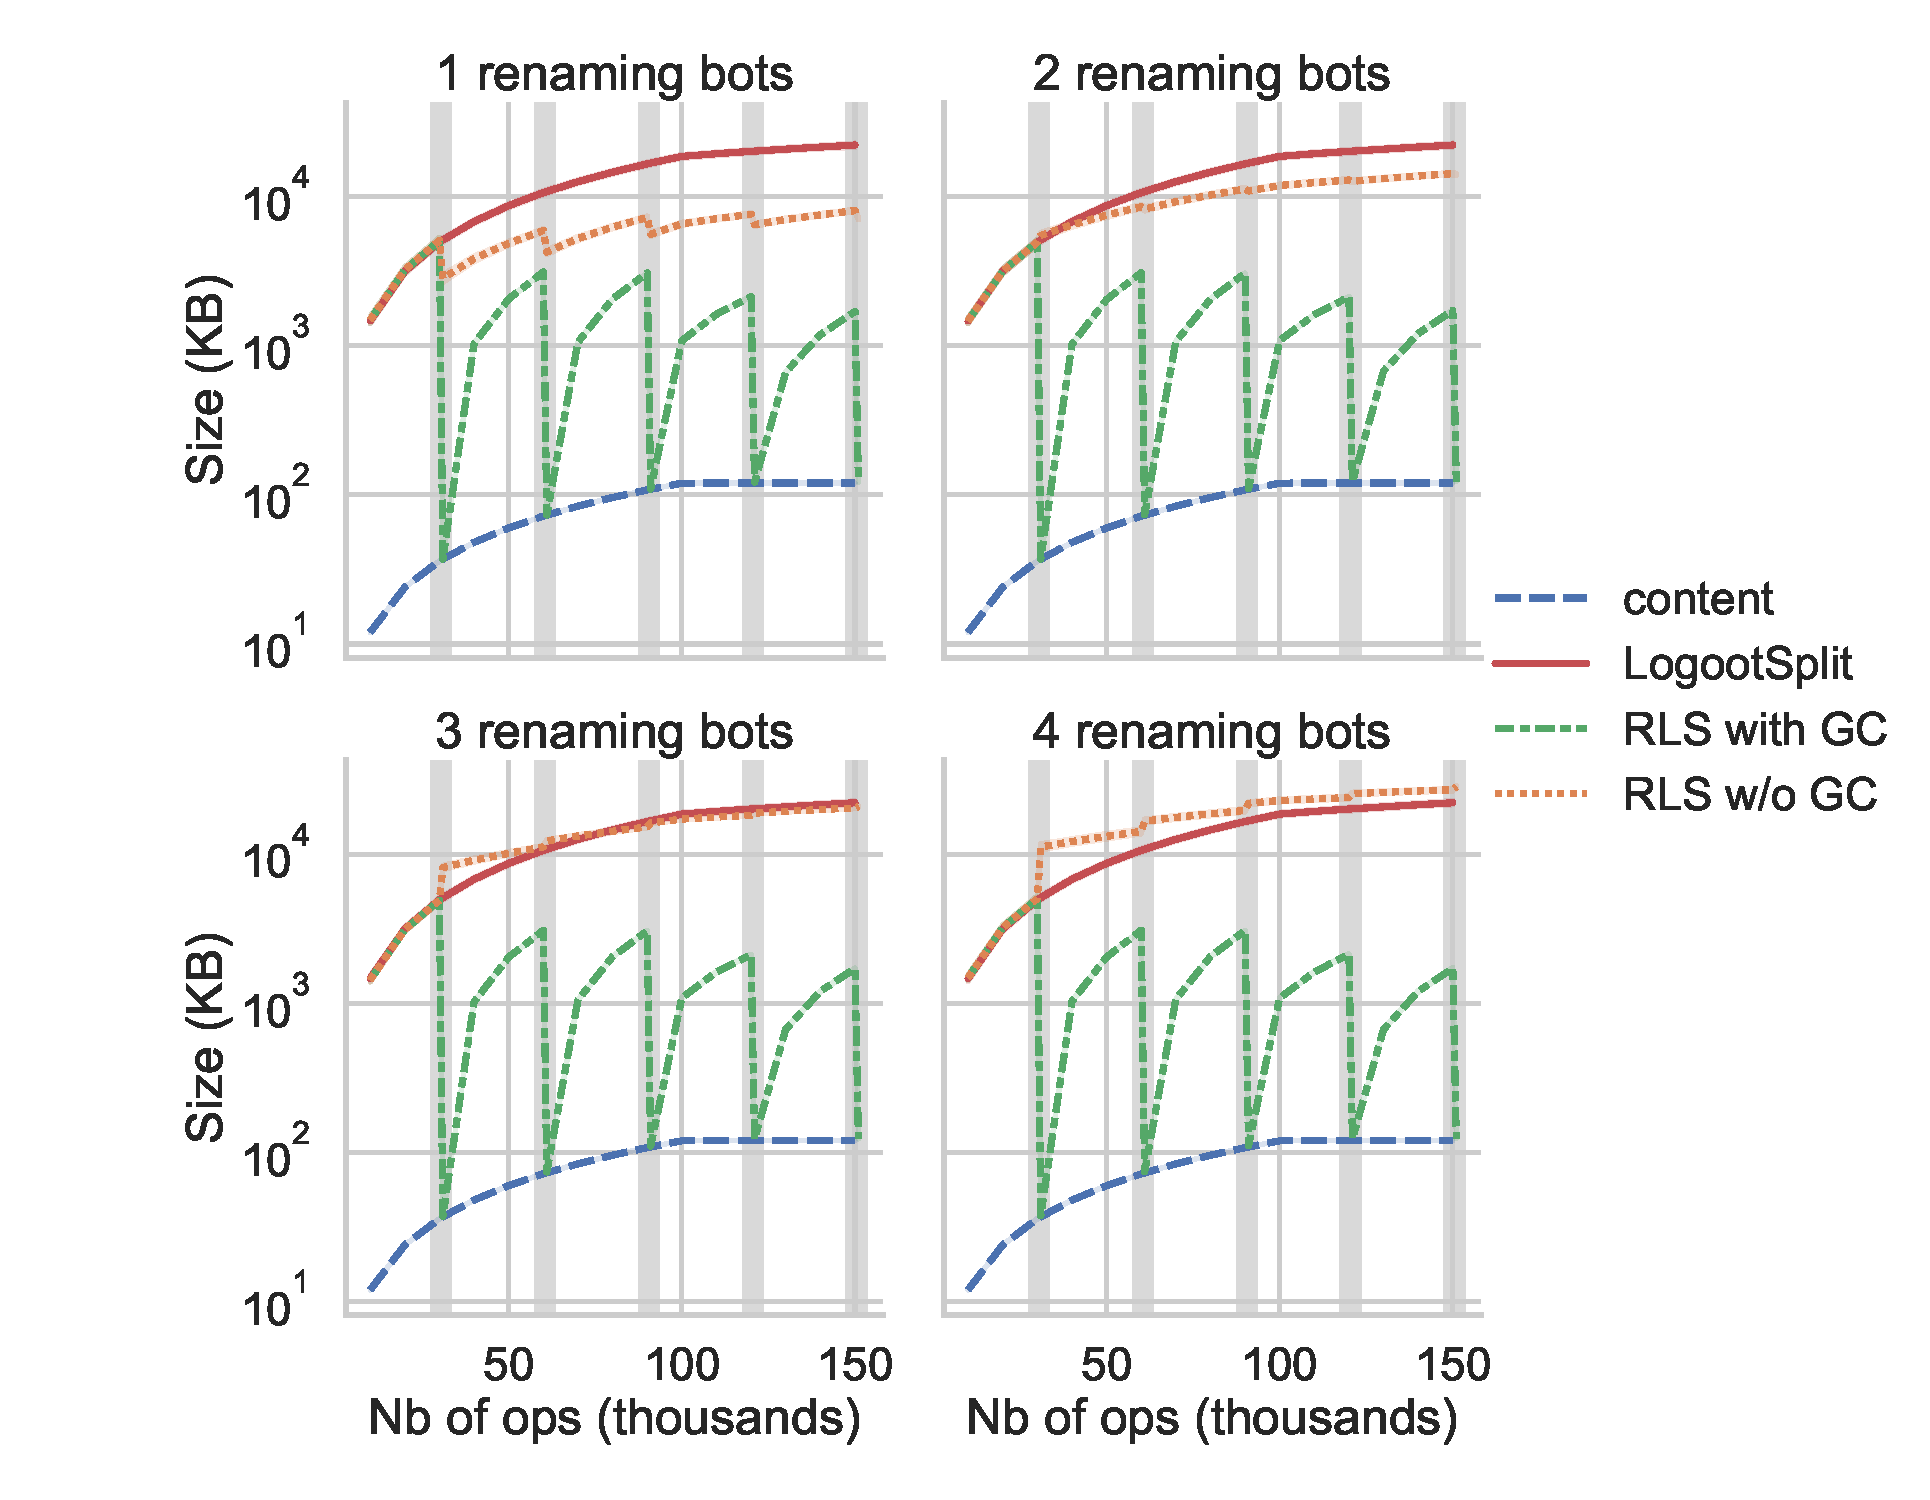
\includegraphics[width=\columnwidth]{img/snapshot-sizes.pdf}
    \caption{Evolution of the size of the document}
    \label{fig:evolution-document-size}
\end{figure}

\begin{itemize}
    \item Display in \autoref{fig:evolution-document-size} the evolution of the size of the document throughout its lifetime
    \item Compare the obtained results according to the number of \emph{renaming bots}, \ie the number of bots authorized to issue \emph{rename} operations
    \item For each diagram, present 4 different data
    \item Blue dashed line represents the size of the content
    \item Red line represents the size of the LogootSplit document
    \item Green dashed-dotted line represents RenamableLogootSplit best-case scenario. In this scenario, nodes assume that \emph{rename} operations become causally stable as soon as nodes received them. Nodes are able to garbage collect metadata introduced by the renaming mechanism, such as the \emph{former states}, instantaneously
    \item Orange dotted line represents RenamableLogootSplit worst-case scenario. In this scenario, nodes assume that \emph{rename} operations never become causally stable. Nodes have thus to store renaming mechanism metadata indefinitely
    \item Observe that RenamableLogootSplit is able to dispose of its overhead eventually, since overhead is garbage collected as \emph{rename} operations become causally stable. And this result is independent of the number of \emph{renaming bots}.
    \item Observe that RenamableLogootSplit still outperforms LogootSplit in its worst-case scenario while the number \emph{renaming bots} remains low (1 or 2). This result can be explained by the fact that the renaming mechanism enable us to scrap as well the overhead of the data structure used in LogootSplit to represents the sequence.
    \item But as the number of concurrent \emph{rename} operations increases, the performances of RenamableLogootSplit decreases as the number of \emph{former states} that nodes have to store to transform operations expand
    \item So a greater number of \emph{renaming bots} may lead to a temporary expanded overhead, but which eventually subsides once causal stability is achieved.
    \item In \autoref{sec:offloading-former-states}, we discuss that \emph{former states} may be offloaded until causal stability is achieved to address the temporary memory overhead
\end{itemize}

\paragraph{Integration times of standard operations}

\begin{figure}[ht!]
    \begin{subfigure}{\columnwidth}
        \centering
        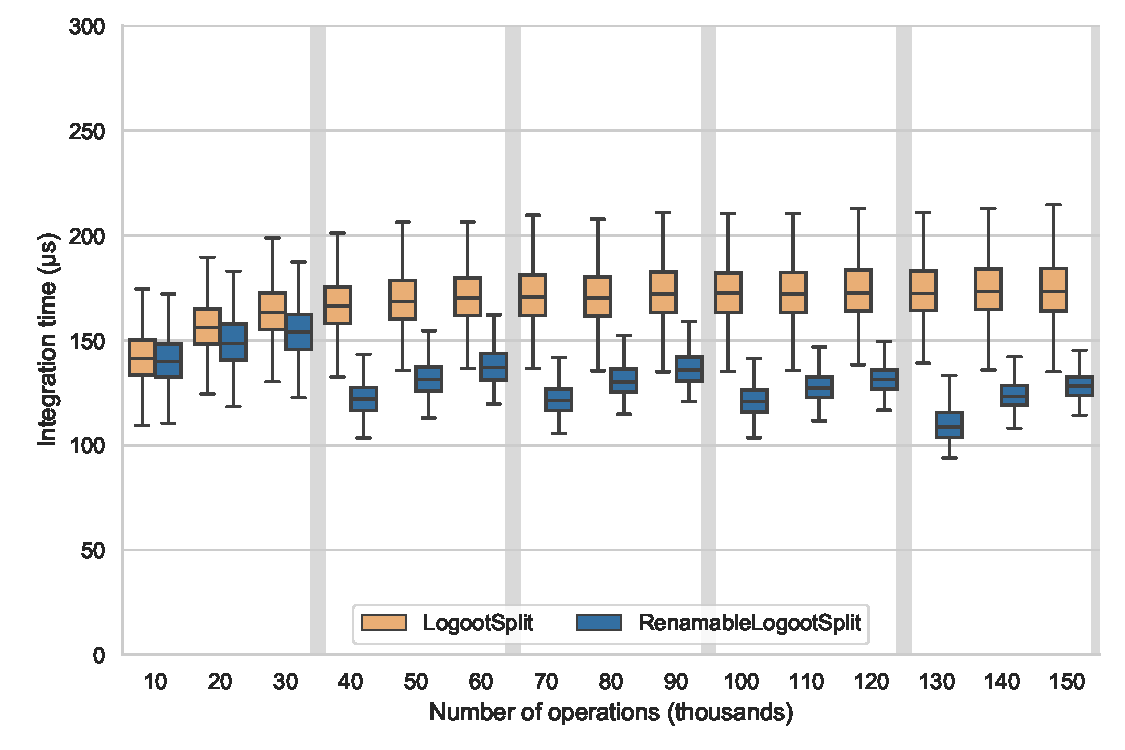
\includegraphics[width=0.9\columnwidth]{img/integration-time-boxplot-local-operations-without-outliers.pdf}
        \caption{Local operations}
        \label{fig:evolution-integration-time-local-insert}
    \end{subfigure}
    \begin{subfigure}{\columnwidth}
        \centering
        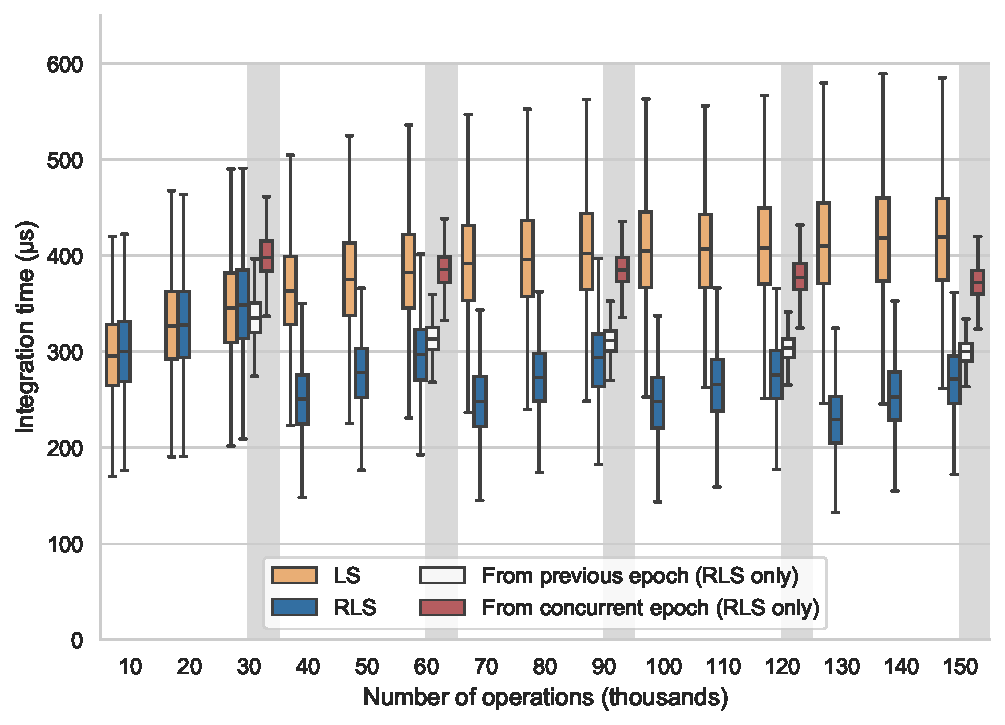
\includegraphics[width=0.9\columnwidth]{img/integration-time-boxplot-remote-operations-without-outliers.pdf}
        \caption{Remote operations}
        \label{fig:evolution-integration-time-remote-insert}
    \end{subfigure}
    \caption{Integration time of standard operations}
    \label{fig:evolution-integration-time-insert}
\end{figure}

\begin{itemize}
    \item In \autoref{fig:evolution-integration-time-insert}, compare the evolution of integration time of respectively local and remote operations on LogootSplit and RenamableLogootSplit documents
    \item Orange boxplots correspond to times on LogootSplit documents while blue ones correspond to times on RenamableLogootSplit documents
    \item Observe that integration times are faster on RenamableLogootSplit, as \emph{rename} operations improve the internal representation of the sequence
    \item In \autoref{fig:evolution-integration-time-remote-insert}, also measure the integration times of remote operations from previous epochs, displayed in white, and of operations from concurrent epochs, displayed in red
    \item Observe a negligible overhead for operations from previous epochs compared to remote operations from the same epochs, as nodes have to rename them beforehand. But still outperforms LogootSplit
    \item Observe an additional overhead for operations from concurrent epochs, as nodes have to reverse the effect of the concurrent epoch first. Achieve performances comparable to LogootSplit ones in this worst-case scenario
\end{itemize}

\paragraph{Integration time of \emph{rename} operation}

\begin{figure}[ht!]
    \centering
    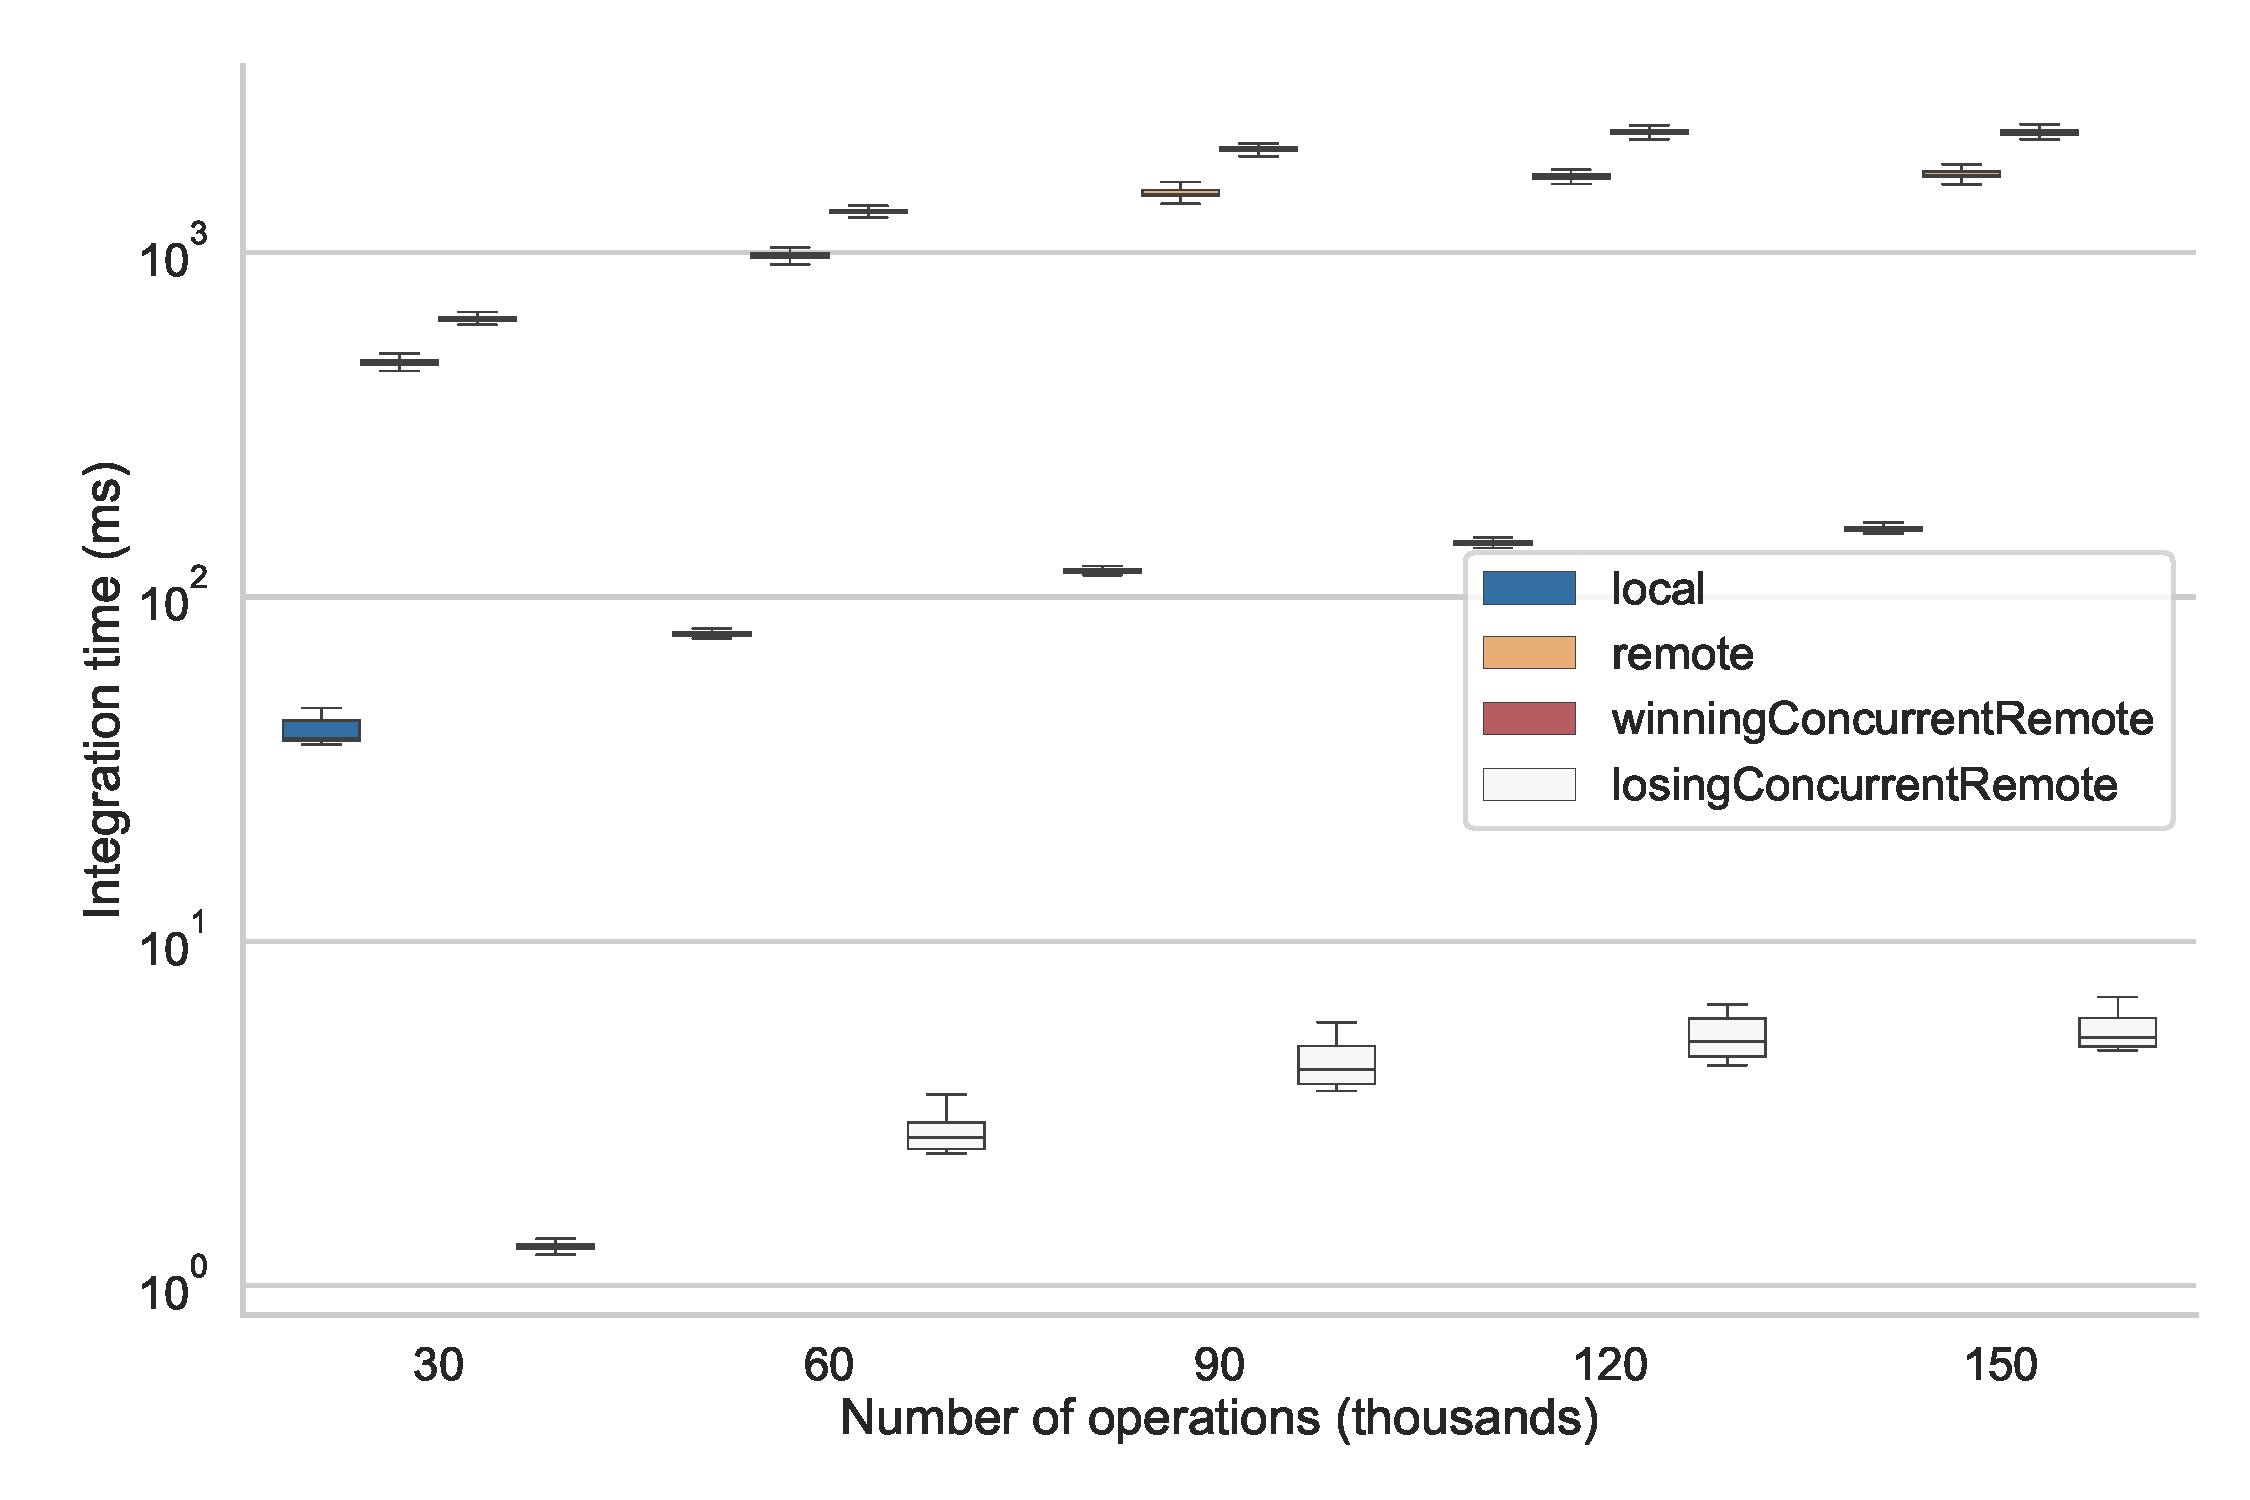
\includegraphics[width=\columnwidth]{img/integration-time-boxplot-rename-op-without-outliers.pdf}
    \caption{Integration time of rename operations}
    \label{fig:evolution-integration-time-rename}
\end{figure}

\begin{itemize}
    \item In figure \autoref{fig:evolution-integration-time-rename}, display integration times of the different kinds of \emph{rename} operations
    \item Main result is that \emph{rename} operations are generally expensive compared to other operations. Local \emph{rename} operations, in blue, takes hundred of milliseconds while remote ones, in orange, may reach seconds if delayed for too long. Should design the strategy to trigger \emph{rename} operations according to this result to prevent a negative impact on the user experience
    \item Another interesting result is that, while \emph{winning rename} operations are expensive to integrate, \emph{losing} ones are cheap. Can thus significantly reduce computations by integrating concurrent \emph{rename} operations in correct order. Will discuss this topic in \autoref{sec:postponing-transition-to-new-epoch}
\end{itemize}

\section{Discussion}

\subsection{Offloading on disk unused \emph{former states}}
\label{sec:offloading-former-states}

\begin{itemize}
    \item \emph{Former states} are only needed to transform operations from previous or concurrent epochs
    \item May receive these kind of operations in 2 cases : \emph{rename} operations are being issued or nodes (re)joined the collaboration
    \item Between these events, \emph{former states} won't actually be needed
    \item Can offload \emph{former states} on disk to reduce the memory overhead until causal stability is achieved, without impacting much performances
\end{itemize}

\subsection{Designing more effective \emph{priority} relation}
\label{sec:designing-more-effective-priority-relation}

\begin{itemize}
    \item While simple and ensuring convergence, the \emph{priority} relation designed and used in this paper introduces a significant computational overhead in some cases
    \item For example a single node, disjoined from the collaboration for a long time, may force every other nodes to revert \emph{rename} operations they issued meanwhile because of its own primary \emph{rename} operation
    \item Should define a \emph{priority} which aims to reduce the global amount of computations of the system, while still ensuring convergence
    \item To this end, could integrate some metrics representing the work done beforehand in \emph{rename} operations
    \item And build a new \emph{priority} relation based on these metrics
\end{itemize}

\subsection{Postponing transition to new epoch in case of high concurrency}
\label{sec:postponing-transition-to-new-epoch}

\begin{itemize}
    \item Primary remote \emph{rename} operations are expensive to integrate as nodes have to browse and rename their whole current state in the process
    \item It can introduce a significant computational overhead in some cases
    \item For example a node may receive concurrent \emph{rename} operations in the reverse order to the one set by the \emph{priority} relation
    \item The node would then consider each operation as the primary one and rename its state in a successive manner
    \item On the other hand, secondary remote \emph{rename} operations are cheap to integrate as nodes simply add to their state a reference to the corresponding \emph{former state}
    \item To reduce the likelihood and the negative impact of the scenario described previously, we can decompose the integration of \emph{rename} operations into two parts in case of concurrency detection
    \item Nodes first process \emph{rename} operations as secondary ones. It enables nodes to integrate remote \emph{insert} and \emph{remove} operations, even from concurrent epochs, by transforming them
    \item Then once nodes obtain a given amount of confidence that one \emph{rename} operation is the primary one, proceed to the renaming of their states
    \item This strategy introduces a slight overhead for each \emph{insert} or \emph{remove} operation received during this period, but reduces the probability of erroneously integrating \emph{rename} operations as primary ones
\end{itemize}

\section{Related work}

\subsection{The core-nebula approach}

\subsection{The LSEQ approach}

\section{Conclusions and future work}

\appendix

\section{Algorithms}

\begin{algorithm}
    \caption{Remaining functions to rename identifier}
    \begin{algorithmic}

    \Function{renIdFromIndex}{$\trm{pos}, \trm{nId}, \trm{nSeq}, \trm{index}$}
        \State \Return $\trm{new Id}(\trm{pos}, \trm{nId}, \trm{nSeq}, \trm{index})$
    \EndFunction
    \\
    \Function{renIdLessThanFirstId}{$\trm{id}, \trm{firstId}, \trm{newFirstId}$}
        \State $\trm{offset} \gets \trm{getLastOffset}(\trm{firstId}) - 1$
        \State $\trm{predOfFirstId} \gets \trm{createIdFromBase}(\trm{firstId}, \trm{offset})$
        \State $\trm{prefix} \gets \trm{concat}(\trm{predOfFirstId}, \trm{MAX\_TUPLE})$
        \State $\trm{predNewFirstId} \gets \trm{createIdFromBase}(\trm{newFirstId}, -1)$

        \If{$\trm{isPrefix}(\trm{prefix}, id)$}
            \State $\trm{tail} \gets \trm{getTail}(\trm{id}, \trm{prefix.length})$
            \State \Return $\trm{concat}(\trm{predNewFirstId}, \trm{tail})$
        \ElsIf{$\trm{id} < \trm{newFirstId}$}
            \State \Return $\trm{id}$
        \Else
            \State \Return $\trm{concat}(\trm{predNewFirstId}, \trm{id})$
        \EndIf
    \EndFunction
    \\
    \Function{renIdGreaterThanLastId}{$\trm{id}, \trm{lastId}, \trm{newLastId}$}
        \State $\trm{prefix} \gets \trm{concat}(\trm{lastId}, \trm{MIN\_TUPLE})$

        \If{$\trm{isPrefix}(\trm{prefix}, id)$}
            \State $\trm{tail} \gets \trm{getTail}(\trm{id}, \trm{prefix.length})$
            \State \Return $\trm{tail}$
        \ElsIf{$\trm{newLastId} < \trm{id}$}
            \State \Return $\trm{id}$
        \Else
            \State \LeftComment{$\trm{lastId} < \trm{id} < \trm{newLastId}$}
            \State \Return $\trm{concat}(\trm{newLastId}, \trm{id})$
        \EndIf
    \EndFunction
    \end{algorithmic}
\end{algorithm}

\begin{algorithm}
    \caption{Remaining functions to reverse rename identifier}
    \begin{algorithmic}

    \Function{revRenIdLessThanNewFirstId}{$\trm{id}, \trm{firstId}, \trm{newFirstId}$}
        \State $\trm{predNewFirstId} \gets \trm{createIdFromBase}(\trm{newFirstId}, -1)$
        \If{$\trm{predNewFirstId} < \trm{id}$}
            \State $\trm{tail} \gets \trm{getTail}(\trm{id}, 1)$
            \If{$\trm{tail} < \trm{firstId}$}
                \State \Return $\trm{tail}$
            \Else
                \State $\trm{offset} \gets \trm{getLastOffset}(\trm{firstId})$
                \State $\trm{predFirstId} \gets \trm{createIdFromBase}(\trm{firstId}, \trm{offset}) $
                \State \Return $\trm{concat}(\trm{predFirstId}, \trm{MAX\_TUPLE}, \trm{tail})$
            \EndIf
        \Else
            \State \Return $\trm{id}$
        \EndIf
    \EndFunction
    \\
    \Function{revRenIdGreaterThanNewLastId}{$\trm{id}, \trm{lastId}$}
        \If{$\trm{id} < \trm{lastId}$}
            \State \Return $\trm{concat}(\trm{lastId}, \trm{MIN\_TUPLE}, \trm{id})$
        \Else
            \State \Return $\trm{id}$
        \EndIf
    \EndFunction
    \end{algorithmic}
\end{algorithm}

\bibliography{ref}

\end{document}
